\chapter{Solving spin-glass problems using tensor networks}
\label{chapter:tn}

Benchmarking quantum annealers requires more sophisticated algorithms.
While there exists a plethora of general-purpose
optimization algorithms, one might hope to achieve better results by exploiting
the topology of the problem's underlying graph and thus locality therein. In
this chapter, we describe a recent, tensor network-based algorithm for finding
low-energy spectrum of Ising spin-glasses, designed for problems defined on
Chimera-like quasi-two-dimensional graphs. The algorithm exploits the sparsity
and locality of the Chimera graph by representing the Boltzmann distribution of
spin-glass as a tensor network, whose approximate contraction can be used for
computing marginal probability distributions. This procedure can then be
combined with the well-known branch and bound algorithm to iteratively select
the most promising partial solutions, finally producing an approximation of the
low-energy spectrum.

\section{Introduction to tensor networks}

\todo[inline,color=SkyBlue]{Mention that the algorithm is physics inspired}
\todo[inline,color=SkyBlue]{Mention the other Chimera-specific algorithm}

\subsection{Branch and bound}
Let us start by considering an Ising spin glass problem defined on a square
lattice, as depicted in Fig. \ref{fig:lattice-and-border}. The state space of
such a system can be viewed as a tree, in which $k$-th level contains all
partial configurations $(s_1, \ldots, s_k)$. This representation allows one to
explore the state space incrementally in search for low energy states, and
possibly prune the less promising branches. In the approach described here, we
use marginal probability $p(s_1, s_2, \ldots, s_k)$ as a criterion for deciding
which partial configurations are most promising. More precisely, we explore the
solution tree in a top-down manner, keeping at most $M$ states at $k$-th level
and branching them into $2M$ new partial configurations at level $k+1$ . The
new marginal probability distributions can be computed as

\begin{figure}
  \centering
  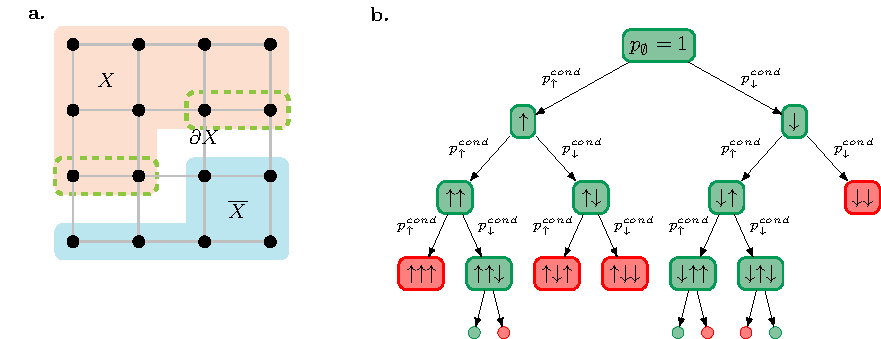
\includegraphics[width=\textwidth]{figures/squarelattice.pdf}
  \caption{\textbf{a.} An example Ising spin--glass  of 16 spins on a square lattice. The conditional probability for spins in the region $\overline{X}$ conditioned with a given configuration of spins in the region $X$ depends only on part of the configuration on the border $\partial X$. \textbf{b.} A fragment of state space tree. States kept at each level
    are marked with green, and the pruned branches are marked with red.}
  \label{fig:lattice-and-border}
\end{figure}

\begin{equation}
  \label{eq:conditional-prob}
  p(s_1, s_2, \ldots, s_k, s_{k+1}) = p(s_1, s_2, \ldots, s_k)p(s_{k+1}|, s_1, \ldots, s_k)
\end{equation}
We can exploit locality of the problem by observing that conditional
probability in \eqref{eq:conditional-prob} of configuration in the region $X =
  (1, 2, \ldots, k)$ depends only on configuration on the border $\partial X$ consisting of those spins, that directly interact with the region
$\overline{X} = (k+1, 2, \ldots N)$. To see that, denote by $H_X$ the usual
    Hamiltonian $H$ restricted to the graph induced by vertices in $X$. Further,
    let $H_{X, \overline{X}} = H - H_X - H_{\overline{X}}$. Notice that $H_{X,
    \overline{X}}$ contains only quadratic terms $J_{ij} s_i s_j$ such that $i \in
  X$ and $j \in \overline{X}$. Slightly abusing the notation, one may thus write
    \begin{equation}
      H(s_1, \ldots, s_N) = H_X(s_1, \ldots, s_k) + H_{\overline{X}}(s_{k+1}, \ldots, s_N) + H_{X, \overline{X}}(s_1, \ldots, s_N)
    \end{equation}
    Using definition of conditional probability applied to Boltzmann distribution,
    one thus gets
    \begin{align}
      p(s_{k+1}|s_1, \ldots, s_k) & = \frac{\sum\limits_{(z_{k+2}, \ldots, z_N)}e^{-\beta H(s_1, \ldots, s_{k+1}, z_{k+2},\ldots,z_N)}}{\sum\limits_{(z_{k+1}, \ldots, z_N)}e^{-\beta H(s_1, \ldots, s_k, z_{k+1},\ldots,z_N)}}                                                                                                                                                     \\
                                  & = \frac{\sum\limits_{(z_{k+2}, \ldots, z_N)}e^{-\beta (H_X(s_1, \ldots, s_k) + H_{\overline{X}}(s_{k+1}, z_{k+2},\ldots,z_N) + H_{X, \overline{X}}(s_1, \ldots, z_N))}}{\sum\limits_{(z_{k+1}, \ldots, z_N)}e^{-\beta (H_X(s_1, \ldots, s_k) + H_{\overline{X}}(z_{k+1}, \ldots,z_N) + H_{X, \overline{X}}(s_1, \ldots, z_N))}}                 \\
                                  & = \frac{e^{-\beta H_X(s_1, \ldots, s_k)}\sum\limits_{(z_{k+2}, \ldots, z_N)} e^{-\beta(H_{\overline{X}}(s_{k+1}, z_{k+2},\ldots,z_N) + H_{X, \overline{X}}(s_1, \ldots, z_N))}}{e^{-\beta H_X(s_1, \ldots, s_k)}\sum\limits_{(z_{k+1}, \ldots, z_N)}e^{ -\beta(H_{\overline{X}}(z_{k+1}, \ldots,z_N) + H_{X, \overline{X}}(s_1, \ldots, z_N))}} \\
                                  & = \frac{\sum\limits_{(z_{k+2}, \ldots, z_N)} e^{-\beta(H_{\overline{X}}(s_{k+1}, z_{k+2},\ldots,z_N) + H_{X, \overline{X}}(s_1, \ldots, z_N))}}{\sum\limits_{(z_{k+1}, \ldots, z_N)}e^{ -\beta(H_{\overline{X}}(z_{k+1}, \ldots,z_N) + H_{X, \overline{X}}(s_1, \ldots, z_N))}}
    \end{align}
    Note, both in numerator and denominator spins with indices from $X$ appear
    non-trivially only in $H_{X, \overline{X}}$ , i.e. the whole expression depends
    only on those spins in $X$ that directly interact with spins in $\overline{X}$,
which was to be demonstrated.

Before discussing how probabilities in \eqref{eq:conditional-prob} can be
computed, let us first extend the above approach to the more general case of a
quasi-two-dimensional graph, i.e. one in which nodes can be grouped into
\emph{clusters} forming a two-dimensional square lattice (see Fig.
\ref{fig:clustering} for details). One can easily see, that again we can construct
a tree-like structure representing state space, this time considering joint
configurations of spins in a single cluster. Therefore, for the most of the
time, we might "forget" the underlying spin-glass structure and consider square
lattices in which spin clusters act like a higher-dimensional systems.

\begin{figure}
  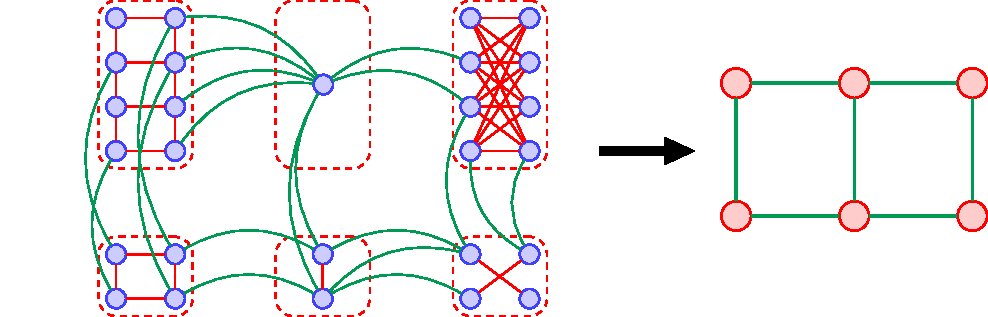
\includegraphics[width=\textwidth]{figures/clustering}
  \caption{Grouping spins into clusters in a Chimera-like graph.}
  \label{fig:clustering}
\end{figure}

A central object considered in our algorithm is the probability distribution
$\exp[-\beta H(\mathbf{s})]$, which we approximate using a PEPS-equivalent
tensor network, whose detail will be described shortly. Contracting such a
network can give the probability distribution of any full configuration, as
well as the marginal probabilities.

\begin{equation}
  p(s_1, s_2, \ldots, s_k) \sim \tr[\mathcal{P}_{(s_1, \ldots, s_k)} e^{-\beta H(\mathbf{s})}]
\end{equation}

\section{Grouping spins into clusters}
The outlined approach can be easily extended to the case of the problem defined
on a graph in which nodes can be grouped into \emph{clusters} forming a
two-dimensional lattice. See Fig. \ref{fig:quasi2d} for a detailed description.
In this more general case, $s_i$ in \eqref{eq:conditional-prob} denote join
probability of configuration in $i$-th cluster, and each configuration is
branched into $2^lM$ new ones, where $l$ is the number of spins in respective
cluster.

\section{PEPS network construction}
We begin construction of a PEPS network for a quasi-two-dimensional graph by
considering two spins at sites $i$ and $j$ connected by an edge $J_{ij}$. This
edge can be decomposed as

\begin{equation}
  e^{-\beta J_{ij}s_i s_j} = \sum_{\gamma = \pm 1} B^{s_{i\phantom{j}}}_\gamma C^{s_j}_\gamma
\end{equation}
where
\begin{equation}
  \label{eq:decomposition}
  B^{S_i}_\gamma = \delta_{\gamma s_i} \quad C^{s_j}_\gamma = e^{-\beta \gamma J_{ij} s_j}
\end{equation}
Note that decomposition \eqref{eq:decomposition}, although not unique, has the
advantage of comprising only non-negative coefficients, which positively
affects numerical stability. Next, with each cluster we associate a PEPS tensor
\begin{equation}
  \label{eq:peps}
  A^{\mathbf{s_c}}_{\mathbf{lrud}} = e^{-\beta H(\mathbf{s_c})} B^{\mathbf{s_c}^l}_\mathbf{l}C^{\mathbf{s_c}^r}_\mathbf{r}B^{\mathbf{s_c}^u}_\mathbf{u}C^{\mathbf{s_c}^d}_\mathbf{d}
\end{equation}
Here, $\mathbf{s_c}$ collects all spins in a given cluster, and
  $\mathbf{s_c}^l$, $\mathbf{s_c}^r$, $\mathbf{s_c}^u$, $\mathbf{s_c}^d$ collect
    spins interacting with it from the left, right, up and down respectively. Each
    such tensor has five legs: the physical one $\mathbf{s_c}$ of dimension $2^m$,
    where $m$ denotes the number of spins in the cluster, and the virtual ones $l,
  r, u, d$ with dimensions depending on the number of inter-cluster edges. Note
    that $H$ in \eqref{eq:peps} is restricted to the graph induced by spins
    belonging to the considered cluster. The construction is depicted in Fig. \ref{fig:tensors}.

    \begin{figure}
      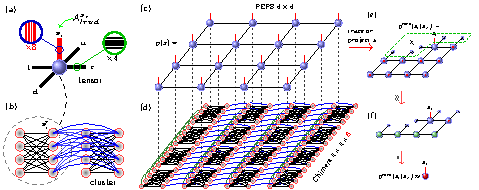
\includegraphics[width=\textwidth]{figures/peps.pdf}
      \caption{Construction of PEPS network}
      \label{fig:tensors}
    \end{figure}



\section{Results}
We benchmarked our algorithm agains classical solvers based on Parallel-Tempering
and D-Wave Quantum annealer DW-2000Q$_6$. As it is hard to directly compare samples
obtained form the D-Wave annealer with output of our deterministic algorithm,
we decided to use time-to-solution as a metric. The results of this benchmarks
is presented in Table \ref{tab:tnvspt}.


\begin{table}
\centering
\begin{tabular}{|l|c|ccc|}
  \hline
\rowcolor{theader}  Method & approx. ratio & $N=512$ & $N=1152$ & $N=2048$ \\
\hline
  TN & g.s. & 30s& 150s & 450s \\
  \hline
\hline
PT (adaptive) & g.s. & 800s & --- & --- \\
\hline
PT (geometric)& $0.01$ & 0.53s & 4.16s & --- \\
PT (geometric)& $0.005$ & 2.51s & 56.4s & --- \\
PT (geometric)& $0.001$ & 158.4s & timed-out & --- \\
PT (geometric)& $0.0001$ & 897.6s & timed-out & --- \\
\hline
\hline
DWave 2000Q$_6$ & $0.01$ & $0.003$s & $0.006$s & $0.02$s \\
DWave 2000Q$_6$ & $0.005$ & $0.2$s & timed-out & timed-out \\
DWave 2000Q$_6$ & $0.001$ & timed-out & timed-out  & timed-out \\
\hline
\hline
\end{tabular}
\caption{Comparison of time-to-solution metric for our tensor network
  based algorithm, in-house parallel tempering implementation and
  D-Wave 2000Q$_{6}$.}
\label{tab:tnvspt}
\end{table}
%%% Local Variables:
%%% mode: latex
%%% TeX-master: "../main"
%%% End:
